\documentclass[12pt,english,french]{article}\usepackage{graphicx, color}
%% maxwidth is the original width if it is less than linewidth
%% otherwise use linewidth (to make sure the graphics do not exceed the margin)
\makeatletter
\def\maxwidth{ %
  \ifdim\Gin@nat@width>\linewidth
    \linewidth
  \else
    \Gin@nat@width
  \fi
}
\makeatother

\IfFileExists{upquote.sty}{\usepackage{upquote}}{}
\definecolor{fgcolor}{rgb}{0.2, 0.2, 0.2}
\newcommand{\hlnumber}[1]{\textcolor[rgb]{0,0,0}{#1}}%
\newcommand{\hlfunctioncall}[1]{\textcolor[rgb]{0.501960784313725,0,0.329411764705882}{\textbf{#1}}}%
\newcommand{\hlstring}[1]{\textcolor[rgb]{0.6,0.6,1}{#1}}%
\newcommand{\hlkeyword}[1]{\textcolor[rgb]{0,0,0}{\textbf{#1}}}%
\newcommand{\hlargument}[1]{\textcolor[rgb]{0.690196078431373,0.250980392156863,0.0196078431372549}{#1}}%
\newcommand{\hlcomment}[1]{\textcolor[rgb]{0.180392156862745,0.6,0.341176470588235}{#1}}%
\newcommand{\hlroxygencomment}[1]{\textcolor[rgb]{0.43921568627451,0.47843137254902,0.701960784313725}{#1}}%
\newcommand{\hlformalargs}[1]{\textcolor[rgb]{0.690196078431373,0.250980392156863,0.0196078431372549}{#1}}%
\newcommand{\hleqformalargs}[1]{\textcolor[rgb]{0.690196078431373,0.250980392156863,0.0196078431372549}{#1}}%
\newcommand{\hlassignement}[1]{\textcolor[rgb]{0,0,0}{\textbf{#1}}}%
\newcommand{\hlpackage}[1]{\textcolor[rgb]{0.588235294117647,0.709803921568627,0.145098039215686}{#1}}%
\newcommand{\hlslot}[1]{\textit{#1}}%
\newcommand{\hlsymbol}[1]{\textcolor[rgb]{0,0,0}{#1}}%
\newcommand{\hlprompt}[1]{\textcolor[rgb]{0.2,0.2,0.2}{#1}}%

\usepackage{framed}
\makeatletter
\newenvironment{kframe}{%
 \def\at@end@of@kframe{}%
 \ifinner\ifhmode%
  \def\at@end@of@kframe{\end{minipage}}%
  \begin{minipage}{\columnwidth}%
 \fi\fi%
 \def\FrameCommand##1{\hskip\@totalleftmargin \hskip-\fboxsep
 \colorbox{shadecolor}{##1}\hskip-\fboxsep
     % There is no \\@totalrightmargin, so:
     \hskip-\linewidth \hskip-\@totalleftmargin \hskip\columnwidth}%
 \MakeFramed {\advance\hsize-\width
   \@totalleftmargin\z@ \linewidth\hsize
   \@setminipage}}%
 {\par\unskip\endMakeFramed%
 \at@end@of@kframe}
\makeatother

\definecolor{shadecolor}{rgb}{.97, .97, .97}
\definecolor{messagecolor}{rgb}{0, 0, 0}
\definecolor{warningcolor}{rgb}{1, 0, 1}
\definecolor{errorcolor}{rgb}{1, 0, 0}
\newenvironment{knitrout}{}{} % an empty environment to be redefined in TeX

\usepackage{alltt}
\usepackage[francais]{babel}
\usepackage[T1]{fontenc}
\usepackage{lmodern}
\usepackage[utf8]{inputenc}
\usepackage{numprint}
\usepackage{url}
\usepackage{makeidx}
\makeindex



\begin{document}

\title{CESU - Travail Véronique Brunstein}
\author{V.Brunstein and JCB}
\date{\today}
\maketitle

\section{Les données}

\begin{knitrout}
\definecolor{shadecolor}{rgb}{0.969, 0.969, 0.969}\color{fgcolor}\begin{kframe}
\begin{verbatim}
##  [1] "Groupe"                                                             
##  [2] "date"                                                               
##  [3] "Numéro"                                                             
##  [4] "Diplôme"                                                            
##  [5] "Date"                                                               
##  [6] "Sexe"                                                               
##  [7] "Lieu.exercice"                                                      
##  [8] "experience.urgence.1...oui.2...non"                                 
##  [9] "Date.debut"                                                         
## [10] "date.fin"                                                           
## [11] "confronté.situation.jamais...1.rarement...2.parfois...3.souvent...4"
## [12] "de.quand.date.dernière.situation.d.urgence"                         
## [13] "de.quand.date.dernière.situation.d.urgence.1"                       
## [14] "formation.urgence"                                                  
## [15] "date.derniere.formation.urgence"                                    
## [16] "A"                                                                  
## [17] "B"                                                                  
## [18] "C"                                                                  
## [19] "D"                                                                  
## [20] "E"                                                                  
## [21] "F"                                                                  
## [22] "G"                                                                  
## [23] "H"                                                                  
## [24] "I"                                                                  
## [25] "J"                                                                  
## [26] "K"                                                                  
## [27] "L"                                                                  
## [28] "M"                                                                  
## [29] "N"                                                                  
## [30] "Q1A"                                                                
## [31] "Q1B"                                                                
## [32] "Q2A"                                                                
## [33] "Q2B"                                                                
## [34] "Q3A"                                                                
## [35] "Q3B"                                                                
## [36] "Q4A"                                                                
## [37] "Q4B"                                                                
## [38] "Q5A"                                                                
## [39] "Q5B"                                                                
## [40] "Q6A"                                                                
## [41] "Q6B"                                                                
## [42] "Q7A"                                                                
## [43] "Q7B"                                                                
## [44] "Q8A"                                                                
## [45] "Q8B"                                                                
## [46] "Q9A"                                                                
## [47] "Q9B"                                                                
## [48] "Tel"
\end{verbatim}
\end{kframe}
\end{knitrout}


\section{Analyse des données}
\subsection{Formation initiale}
\begin{knitrout}
\definecolor{shadecolor}{rgb}{0.969, 0.969, 0.969}\color{fgcolor}\begin{kframe}
\begin{verbatim}
##         AS        IDE SAGE FEMME 
##          3         16          1
\end{verbatim}
\end{kframe}
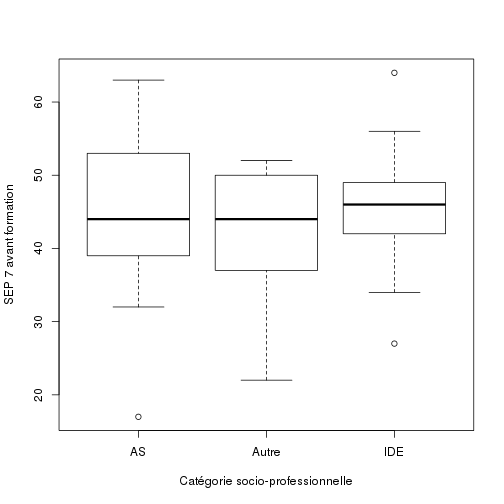
\includegraphics[width=\maxwidth]{../figure/unnamed-chunk-4} 

\end{knitrout}



\section{Echelle de Likert}

Pour chaque item de l'echelle de Likert, on présente:
\begin{itemize}
  \item une représentation graphique de l'echelle avant/après
  \item une comparaison des deux moyennes au moyen du test t de Student pour séries appariées. Une différence entre les moyennes avant/après est considérée comme significative lorsque la probabilité d'observer une telle différence (p) est inférieure à $0.05$, c'est à dire trop petite pour que cette différence soit due au hasard.
\end{itemize}

Les réponses aux questions se font sur une échelle allant 1 à 8, ce qui impose une zone de "neutralité" quelque part entre 4 et 5 sans que l'on puisse donner une valeur précise puisque les unités sont entières. Par convention, les opinions négatives correspondent aux valeurs basses de l'échelle (et donc à gauche sur un axe croissant) alors que les opinions positives répondent aux valeurs les plus élevées de l'échelle (et donc à droite sur un axe croissant).

Il existe de nombreuses manières de représenter graphiquement une échelle de Likert. N.B. Robbins et coll. après une analyse critique des représentations possibles recommandent d'utiliser la méthode des graphiques en barre empilées divergentes \cite{1}.
La zone neutre coincide avec la ligne verticale zéro. Tous ceux qui sont plutôt d'accord sont représenté à droite du zéro et dans des tons bleus dont l'intensité croit avec l'accord. Ceux qui sont en désaccord avec la proposition figurent à gauche du zéro et dans des tons rouges d'intensité croissante. Les couleurs ont été choisies pour convenir aux personnes déficientes visuelles. Les réponses sont automatiquement ajustées par rapport à cette ligne de référence ce qui permet de mesurer visuellement l'évolution du groupe.

\subsection{Question Q1}



Avant (Q1A):
\begin{knitrout}
\definecolor{shadecolor}{rgb}{0.969, 0.969, 0.969}\color{fgcolor}\begin{kframe}
\begin{verbatim}
##    Min. 1st Qu.  Median    Mean 3rd Qu.    Max. 
##     4.0     5.0     5.0     5.3     6.0     7.0
\end{verbatim}
\end{kframe}
\end{knitrout}

\begin{enumerate}
  \item \textbf{Min}imum = 4: une partie des personnes ont une opinion plutôt négative sur la proposition.
  \item \textbf{1st. Qu}artile = 5: Le premier quartile (appelé aussi Q25) est à 5 ce qui signifie que 25\% des répondants ont une opinion négative ou neutre sur la proposition.
  \item \textbf{Mediane} = 5: la médiane (appelée aussi Q50) correspond au deuxième quartile, c'est à dire que 50\% des répondants ont une opinion négative ou neutre et 50\% ont une opinion positive ou neutre.
  \item \textbf{Mean} = $5.3$: la moyenne des réponses est égale à $5.3$. Les chiffres décimaux sont toujours délicats à interpréter avec des valeurs entières. La proximité de la moyenne et de la médiane est un indice en faveur de la normalité des valeurs. Si les valeurs sont normales (c'est à dire qu'elles se répartissent comme une courbe de Gauss), ont peut utiliser des tests statistiques paramétriques comme le test de Student pour comparer deux moyennes (dans le cas contraire il faudrait utiliser des tests non paramétriques).
  \item \textbf{3rd. Qu}artile = 6: le troisième quartile (appelé aussi Q75) est égal à 6. Le troisième quartile correspond à 75\% des réponses. L'intervalle interquartile (entre Q25 et Q75) est faible. Globalement on peut dire que les personnes interrrogées ont une opinion neutre à modérément favorable par rapport à la question mais l'enthousiasme est faible.
  \item \textbf{max}imum = 7: quelque personnes sont assez d'accord avec la proposition, mais personne n'a coché le score maximal.
\end{enumerate}

Après (Q1B):
\begin{knitrout}
\definecolor{shadecolor}{rgb}{0.969, 0.969, 0.969}\color{fgcolor}\begin{kframe}
\begin{verbatim}
##    Min. 1st Qu.  Median    Mean 3rd Qu.    Max. 
##    6.00    7.00    7.00    7.05    7.25    8.00
\end{verbatim}
\end{kframe}
\end{knitrout}

Après la formation l'opinion du groupe à évoluée positivement. Toutes les opinions sont franchement favorables et personne ne se situe dans la zone de neutralité(\textbf{Min}imum = 6). Le score maximal est atteint (\textbf{max}imum = 8) et le troisième quartile (q75 = $7.5$) atteint presque le score maximal.

Graphiquement, cette évolution est bien visible (fig.\ref{Q1_likert}). La courbe des réponses se décale vers la droite tandis que les nuances de bleu se renforcent (Q1B) traduisant une forte augmentation des opinions positives.

Il y a une différence significative entre les moyennes des scores avant et après, que l'on peut objectiver avec un test de Student pour séries appariées. L'hypothèse neutre que l'on pose à priori est qu'il n'existe pas d'évolution dans l'opinion du groupe et que la différence avant/après est due au hasard. L'hypothèse alternative est qu'au contraire, il y a une évolution dans l'opinion du groupe. Le test statistique évalue l'hypothèse neutre  et le résultat obtenu amène à rejeter l'hypothèse neutre (la différence avant/après n'est pas due au hasard) et par conséquent d'accepter l'hypothèse alternative.

($t(19)=-8.097$,
$p < 0.001$).
(Voir figure \ref{Q1_box} page \pageref{Q1_box}).
La valeur p indique que l'on a moins d'une chance sur $1000$ de se tromper en affirmant que l'hypothèse neutre est fausse.

\begin{figure}
\begin{center}
\begin{knitrout}
\definecolor{shadecolor}{rgb}{0.969, 0.969, 0.969}\color{fgcolor}
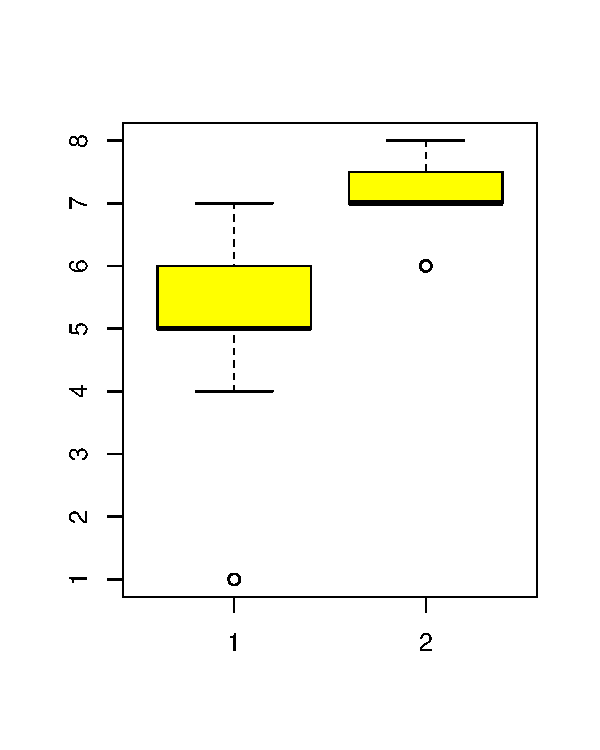
\includegraphics[width=\maxwidth]{figure/Q1_boxplot} 

\end{knitrout}

\end{center}
\caption{Représentation sous forme de "boite à moustaches" (box-plot) de l'évolution des opinions pour la question Q1 - Avant/Après. Les rectangles jaunes correspondent à la distance interquartile (Q25-Q75) et le trait épais à la médiane. On observe que non seulement les opinions ont évolués positivement mais que l'opinion du groupe est plus consensuelle (rectangle plus petit). L'absence de chevauchement des deux rectangles indique que la différence avant/après sera statistiquement significative.}
\label{Q1_box}
\end{figure}




\begin{figure}
\begin{center}
\begin{knitrout}
\definecolor{shadecolor}{rgb}{0.969, 0.969, 0.969}\color{fgcolor}
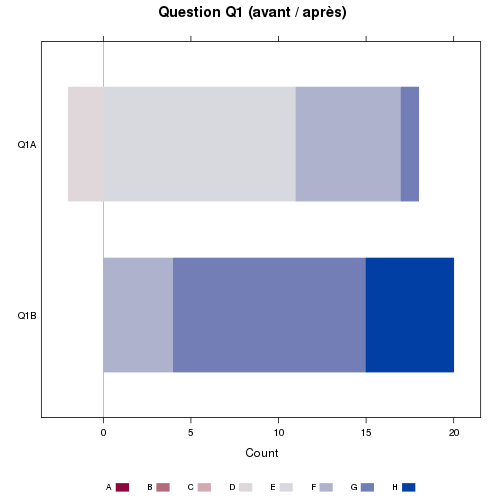
\includegraphics[width=\maxwidth]{../figure/unnamed-chunk-10.png} 

\end{knitrout}

\end{center}
\caption{Evolution des opinions pour la question Q1 - Avant/Après. L'évolution fortement positive du groupe se traduit par un renforcement des nuances de bleu pour la question Q1B et le décalage de la courbe vers la droite. En abscisse figure la taille du groupe (count).}
\label{Q1_likert}
\end{figure}

\bibliographystyle{plain} 
\bibliography{biblio}

\end{document}
